% !TEX program=lualatex
\RequirePackage{luatex85}
\documentclass[11pt,tikz]{standalone}
\usepackage[utf8]{inputenc}
\usepackage[T1]{fontenc}
\usepackage{textcomp}
\usepackage[scaled]{helvet}
\usepackage{tikz}
\usetikzlibrary{shapes,arrows,positioning}
\renewcommand{\familydefault}{\sfdefault}

\begin{document}
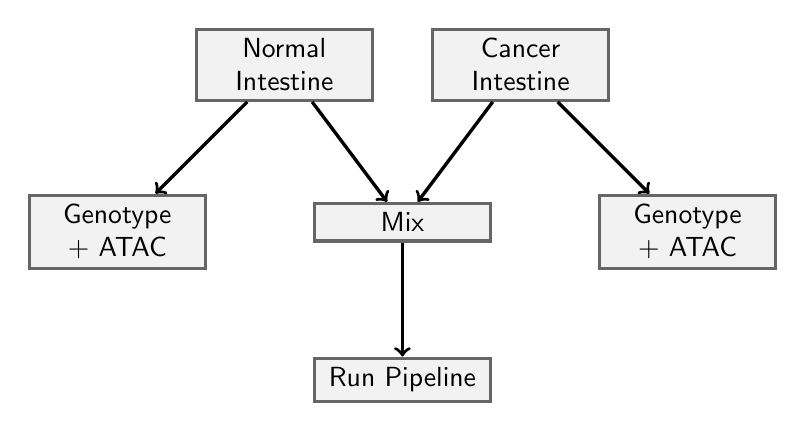
\begin{tikzpicture}[node distance=30mm, text width = 20mm, align = center,auto]
\tikzstyle{line}=[draw, ->, very thick]
\tikzstyle{cir}=[rectangle,draw=black!60,fill=black!5,very thick,on grid]

% \draw[step=1cm,gray,very thin] (-10,-30) grid (20,10);

\node[cir] (norm) {Normal Intestine};
\node[cir, right = of norm] (cancer) {Cancer Intestine};
\node[cir, below right = of cancer] (cgt) {Genotype + ATAC};
\node[cir, below left = of norm] (ngt) {Genotype + ATAC};
\node[cir, below right = 2 and 1.5 of norm] (combo) {Mix};
\node[cir, below = 2 of combo] (pipeline) {Run Pipeline};

\draw[line] (norm) -- (ngt);
\draw[line] (norm) -- (combo);
\draw[line] (cancer) -- (cgt);
\draw[line] (cancer) -- (combo);
\draw[line] (combo) -- (pipeline);

\end{tikzpicture}
\end{document}